\documentclass[11pt]{article}

\usepackage[a4paper,margin=1in]{geometry}
\usepackage[T1]{fontenc}
\usepackage[utf8]{inputenc}
\usepackage{lmodern}
\usepackage{microtype}
\usepackage{amsmath,amssymb}
\usepackage{booktabs}
\usepackage{multirow}
\usepackage{array}
\usepackage{graphicx}
\usepackage{xcolor}
\usepackage{caption}
\usepackage{subcaption}
\usepackage{float}
\usepackage{hyperref}
\usepackage{enumitem}
\usepackage{longtable}
\usepackage{pdflscape}
\usepackage{pgfplots}
\pgfplotsset{compat=1.18}

\hypersetup{
    colorlinks=true,
    linkcolor=blue!60!black,
    citecolor=blue!60!black,
    urlcolor=blue!60!black
}

\graphicspath{{figures/}}

\title{\textbf{Cost-Aware Adaptive Rate Limiting with PPO: Reward Alignment, Budget Utilisation, and Robustness Assessment}}
\author{Harshal Rudra(MT2025706), Manzil Baruah(MT2025715), Sunil Joshi(MT2025726)}
\date{}

\begin{document}
\maketitle

\begin{abstract}
Modern API gateways must regulate admission under limited capacity while balancing three competing objectives: sustaining throughput, keeping latency low, and protecting high-priority traffic. This project begins from a class-based reinforcement learning rate limiter trained with Proximal Policy Optimization (PPO), and extends it to a cost-aware admission-control setting in which each request carries a computational service cost and the server capacity is modeled as a per-step processing budget rather than a fixed request count. The central technical challenge was reward alignment. A naive cost-aware reward, which retained request-count throughput and added only a small processed-cost bonus, caused the policy to collapse into an under-serving regime. Replacing the throughput term with a cost-served objective stabilized learning and produced a high-utilisation policy that used almost all available budget. Across standard traffic scenarios, the resulting cost-aware PPO traded raw request throughput for substantially higher cost efficiency and remained competitive with strong hand-crafted baselines. It generalized well to a cheap-flood out-of-distribution scenario, but still failed under an expensive-attack shift in which a few extremely costly requests monopolized capacity. The overall lesson is that reward engineering is decisive in constrained RL systems, and domain-aware heuristics remain difficult baselines to beat.
\end{abstract}

\section{Introduction}
API gateways are the front line of modern distributed systems. They absorb bursty traffic, enforce fairness, and protect downstream services from overload. A rate limiter that is too permissive creates queues, unstable latency, and wasted retries; one that is too conservative drops useful traffic and reduces service quality. The problem becomes harder when requests have different priorities. Authentication, payment, or model-serving calls often carry higher business importance than logging or analytics requests, so a gateway should not treat all dropped requests equally.

Classical rate-limiting mechanisms such as fixed thresholds and token buckets are robust, lightweight, and easy to deploy, but they are not naturally adaptive to changing traffic patterns. When traffic oscillates, spikes, or carries non-trivial retry behavior, a static controller must rely on hand-tuned rules that may not transfer across workloads. Reinforcement learning is attractive in this setting because it turns rate limiting into sequential decision-making: an agent observes system state, adjusts the admission rate, and learns from resulting throughput, latency, and drops.

The missing ingredient in many simplified RL rate-limiting environments is request heterogeneity. In real systems, API calls are not homogeneous units. A lightweight metadata lookup and a large model inference request should not consume the same portion of the gateway's effective capacity. This project addresses that gap by extending a count-based PPO rate limiter into a cost-aware admission-control environment. Each request now carries a computational service cost, service capacity becomes a processing budget, and the agent must learn to reason about both priority and cost.

The goals of this project are threefold. First, to study reward design in the original count-based setting and understand how penalty weights shape learned behavior. Second, to implement a cost-aware extension that preserves the existing PPO training pipeline as much as possible. Third, to compare the resulting learned policies against strong heuristics and to evaluate robustness under out-of-distribution cost shifts. The rest of the report follows this progression: environment and formulation, methods, experiments, discussion, and conclusions.

\section{Environment and Problem Formulation}
\subsection{Traffic Generator and Scenarios}
The simulator models request arrivals in discrete time. Each episode consists of $180$ timesteps. At every timestep, a scenario-specific stochastic arrival process generates a batch of requests. The main training and evaluation scenarios are:

\begin{itemize}[leftmargin=1.5em]
    \item \textbf{low\_load}: a lightly loaded regime with mean arrival intensity below service capacity.
    \item \textbf{high\_load}: a sustained overload regime with mean intensity well above capacity.
    \item \textbf{bursty}: a moderate baseline load punctuated by short bursts.
    \item \textbf{oscillating}: a periodically varying load with sinusoidal intensity changes.
\end{itemize}

The standard count-based environment was trained on a weighted mixture of these scenarios so that the agent experienced both stable and dynamic traffic. For cost-aware experiments, the same scenario structure was retained.

\subsection{Priority Labels and Retry Dynamics}
Each arriving request is assigned one of three priority classes: high, medium, or low. The environment uses fixed class probabilities during standard training, and each class has its own retry probability. When a request is dropped, it may be retried after a bounded delay. This creates realistic congestion feedback: bad admission decisions not only lose requests immediately but can also amplify future load through retries.

\subsection{Queueing and Service Discipline}
Accepted requests enter a single priority-aware FIFO queue. The service policy itself is not learned. Instead, requests are always served in priority order, and within each priority class they preserve arrival order. This choice isolates the admission-control problem: the novelty in this project is not a new scheduler, but a better controller for how aggressively requests should be admitted under changing demand.

\subsection{Standard Count-Based Control}
In the original environment, the server could process up to $12$ requests per timestep. The agent controlled a rate limit $L_t$ bounded within $[2,18]$. At each timestep the action space consisted of three discrete choices:
\[
a_t \in \{\texttt{decrease},\ \texttt{hold},\ \texttt{increase}\}.
\]
The action changed the rate limit in fixed steps of size $2$. Requests beyond the current rate limit were dropped immediately.

\subsection{Cost-Aware Extension}
The novel environment augments each request with a service cost:
\[
c_i \sim \mathcal{U}(1,5).
\]
This cost remains attached to the request for its entire lifetime. The fixed request-count capacity is replaced by a per-step processing budget:
\[
B = 24.
\]
At each timestep the queue is served greedily in priority-first FIFO order while the remaining budget permits. A request with cost $c_i$ is served only if $c_i \leq B_{\text{remaining}}$. The service loop stops when no next queued request fits into the remaining budget.

This change converts the problem from count-based admission control into a resource-allocation problem. The controller must now learn that two cheap requests may be preferable to one expensive request if both options compete for limited budget.

\subsection{State Representation}
The original state summarized queue length, recent drop behavior, current rate limit, and recent arrivals. The cost-aware state preserved those signals and added cost-sensitive features, including:

\begin{itemize}[leftmargin=1.5em]
    \item total queued service cost,
    \item mean queued service cost,
    \item queued cost for each priority class,
    \item recent arrival cost,
    \item rejected cost from the previous step.
\end{itemize}

All features were normalized to stable ranges so the PPO network could train without pathological scale differences.

\subsection{Reward Formulation}
The original count-based reward used a weighted sum of normalized throughput and penalties:
\begin{equation}
r_t^{\text{count}} =
w_{\text{thr}}\tilde{T}_t
- w_{\text{lat}}\tilde{L}_t
- w_{\text{drop}}\tilde{D}_t
- w_{\text{hp}}\tilde{D}^{H}_t
- w_{\text{ov}} O_t ,
\end{equation}
where $\tilde{T}_t$ is normalized served request count, $\tilde{L}_t$ is normalized latency, $\tilde{D}_t$ is overall drop rate, $\tilde{D}^{H}_t$ is high-priority drop rate, and $O_t$ is an overload indicator.

The first cost-aware attempt kept the count-based throughput term and added only a small bonus for processed cost:
\begin{equation}
r_t^{\text{naive-cost}} =
w_{\text{thr}}\tilde{T}_t
+ w_{\text{cost}}\tilde{C}_t
- w_{\text{lat}}\tilde{L}_t
- w_{\text{drop}}\tilde{D}_t
- w_{\text{hp}}\tilde{D}^{H}_t
- w_{\text{ov}} O_t.
\end{equation}
This proved misaligned: the environment constrained service by cost, but the agent was still primarily rewarded for request count.

The final cost-only reward removed the count-throughput term:
\begin{equation}
r_t^{\text{cost-only}} =
w_{\text{cost}}\tilde{C}_t
+ w_{\text{util}} U_t
- w_{\text{lat}}\tilde{L}_t
- w_{\text{drop}}\tilde{D}_t
- w_{\text{hp}}\tilde{D}^{H}_t
- w_{\text{ov}} O_t ,
\end{equation}
where $\tilde{C}_t$ is normalized served cost and $U_t$ is budget utilization. In the final successful configuration, $w_{\text{thr}}=0$, $w_{\text{cost}}=1.5$, and $w_{\text{util}}=0$ because processed cost already captured the useful work performed by the gateway.

\section{Methods}
\subsection{PPO Agent}
The learning algorithm is PPO with a shared actor-critic network. The network consists of two hidden layers of width $48$ with $\tanh$ activations. The actor outputs a categorical distribution over the three rate-limit actions; the critic estimates the state value. Advantage estimation uses Generalized Advantage Estimation (GAE):
\begin{equation}
\hat{A}_t = \delta_t + \gamma \lambda \hat{A}_{t+1},
\qquad
\delta_t = r_t + \gamma V(s_{t+1}) - V(s_t).
\end{equation}
The PPO objective clips the policy-ratio update:
\begin{equation}
\mathcal{L}_{\text{PPO}} =
\mathbb{E}\left[
\min\left(
\rho_t \hat{A}_t,\;
\text{clip}(\rho_t, 1-\epsilon, 1+\epsilon)\hat{A}_t
\right)
\right].
\end{equation}

The main hyperparameters used throughout the project are shown in Table~\ref{tab:hyperparams}. The action space remained unchanged in all experiments: decrease, hold, or increase the rate limit.

\begin{table}[H]
\centering
\caption{Core PPO and environment hyperparameters used in the main experiments.}
\label{tab:hyperparams}
\begin{tabular}{ll}
\toprule
Parameter & Value \\
\midrule
Episode length & $180$ \\
Rate-limit range & $[2,18]$ \\
Rate step & $2$ \\
Count-based service capacity & $12$ requests/step \\
Cost-aware service budget & $24$ cost units/step \\
Hidden size & $48$ \\
Actor learning rate & $0.005$ \\
Critic learning rate & $0.008$ \\
Discount factor $\gamma$ & $0.97$ \\
GAE parameter $\lambda$ & $0.93$ \\
PPO clip $\epsilon$ & $0.2$ \\
Update epochs & $8$ \\
Minibatch size & $128$ \\
Standard training length & $260$ episodes \\
Evaluation length & $24$ episodes/scenario \\
\bottomrule
\end{tabular}
\end{table}

\subsection{Baselines}
The project includes both count-blind and cost-aware baselines.

\paragraph{Count-blind heuristics.}
These include a fixed rate, a token bucket, an adaptive threshold controller, and a priority heuristic that adjusts limits based on queue pressure.

\paragraph{Cost-aware heuristics.}
For the cost-aware extension, the baselines were adapted so that their thresholds are interpreted against expected cost-budget pressure rather than raw request counts. Two especially relevant baselines are:
\begin{itemize}[leftmargin=1.5em]
    \item \textbf{CostAwarePriority}: a priority-sensitive controller that throttles more aggressively when queued cost grows.
    \item \textbf{CostEfficiency}: a heuristic that implicitly favors requests with better priority-to-cost trade-offs.
\end{itemize}

These baselines are strong because they encode domain structure explicitly. A key goal of the project was to determine whether PPO could discover similar trade-offs from interaction alone.

\subsection{Reward-Design Process}
Reward design became the central scientific story of the project.

\paragraph{Original count-based reward.}
The earliest count-based PPO used a heavy high-priority drop penalty ($w_{\text{hp}}=3.1$). This produced an over-conservative policy that protected important requests by admitting too little traffic overall.

\paragraph{Balanced count-based reward.}
Reducing the high-priority penalty to $1.0$ restored a much healthier operating point. Throughput increased, latency fell, and drop rate improved simultaneously.

\paragraph{Naive cost-aware reward.}
When the environment was made cost-aware, the first reward kept request-count throughput and added only a small processed-cost bonus. This misalignment caused mid-training collapse: the agent learned that raising the rate limit was risky, over-used the decrease action, and eventually under-served almost everything.

\paragraph{Cost-only reward.}
The successful fix was to replace request-count throughput with processed cost as the primary positive signal. This directly aligned the optimization target with the budget-constrained environment. The resulting policy used nearly all available budget and remained stable through the full run.

\paragraph{Fine-tuning.}
A final targeted fine-tuning stage specialized the cost-aware PPO on the \texttt{high\_load} scenario for $30$ additional episodes at slightly higher learning rates. The result gave a modest in-distribution gain but did not close the gap to the strongest heuristics and slightly hurt out-of-distribution robustness.

\paragraph{Warm-start from heuristics.}
The final extension explored imitation-based warm-starting. A strong cost-aware heuristic (\texttt{cost\_aware\_priority}) was used as a teacher to generate demonstration trajectories across the standard training scenarios. The PPO actor-critic network was then pre-trained with behavioral cloning (cross-entropy for actions, mean squared error for critic targets using Monte Carlo returns). Direct PPO fine-tuning from this cloned checkpoint was unstable and destroyed the cloned policy, so a behavior-regularized PPO variant was implemented. During PPO updates, the actor received an additional teacher-action log-probability bonus with weight $\lambda$, anchoring the policy to the safe behavioral region discovered by cloning.

\subsection{Evaluation Methodology}
Performance was measured with:
\begin{itemize}[leftmargin=1.5em]
    \item throughput,
    \item latency,
    \item drop rate,
    \item high-priority success rate,
    \item total served cost,
    \item budget utilization,
    \item total reward.
\end{itemize}

In addition to the standard four traffic scenarios, three cost-shift out-of-distribution (OOD) scenarios were introduced:
\begin{itemize}[leftmargin=1.5em]
    \item \textbf{cheap\_flood}: many very cheap low-priority requests,
    \item \textbf{expensive\_attack}: highly costly high-priority requests,
    \item \textbf{mixed\_shift}: all classes experience unseen cost distributions.
\end{itemize}

A final transfer test used a production-derived cost distribution from the public Azure Functions Invocation Trace 2021. A $500{,}000$-row sample of invocation durations was extracted from the official two-week trace, fitted with a log-normal model for inspection, then scaled into the simulator's integer cost space so that the median duration mapped to cost $3$. The resulting empirical distribution was clipped to the range $[1,15]$ and used as a direct replacement for the synthetic $\mathcal{U}(1,5)$ request-cost sampler. This gave a zero-shot robustness test for policies trained entirely on synthetic costs.

Because the environment is simulation-heavy and the model is small, the project used an efficient screening protocol on CPU rather than long MPS/GPU runs. Short screening runs, validation checkpoints, and early stopping were used to prune bad reward settings before running full experiments.\footnote{One intermediate comparison was invalidated because a global reward default was accidentally changed, causing the baseline and variant to share the same throughput weight. That contaminated result was discarded and rerun with isolated configuration overrides. This is noted explicitly because reproducibility mattered throughout the project.}

\section{Experiments and Results}
\subsection{Weight Ablation on Count-Based PPO}
Table~\ref{tab:count_ablation} summarizes the most important reward-weight ablation in the original count-based setting. The key observation is that the heavy high-priority penalty cripples the agent. Reducing it restores balance, while increasing the throughput weight produces the largest scalar reward.

\begin{table}[H]
\centering
\caption{High-load comparison for count-based PPO reward ablations. The original high-priority penalty ($3.1$) is overly conservative; lower penalty and higher throughput emphasis both recover much stronger operating points.}
\label{tab:count_ablation}
\resizebox{\textwidth}{!}{
\begin{tabular}{lcccccc}
\toprule
Variant & Train Reward Mean & High-Load Reward & Throughput & Latency & Drop Rate & HP Success \\
\midrule
Baseline-Count ($w_{hp}=3.1$) & $-0.332$ & $-120.824$ & $8.587$ & $3.004$ & $0.411$ & $0.830$ \\
PPO-Count-HP1.0 & $0.292$ & $128.383$ & $11.654$ & $1.111$ & $0.208$ & $0.898$ \\
PPO-Count-Throughput2.0 & $0.766$ & $168.770$ & $11.388$ & $2.703$ & $0.214$ & $0.894$ \\
\bottomrule
\end{tabular}
}
\end{table}

Figure~\ref{fig:count_ablation_bars} visualizes the throughput and high-priority success trade-off. The original baseline loses both on throughput and reliability, while the two adjusted rewards produce viable policies.

\begin{figure}[H]
\centering
\begin{subfigure}[t]{0.48\textwidth}
\centering
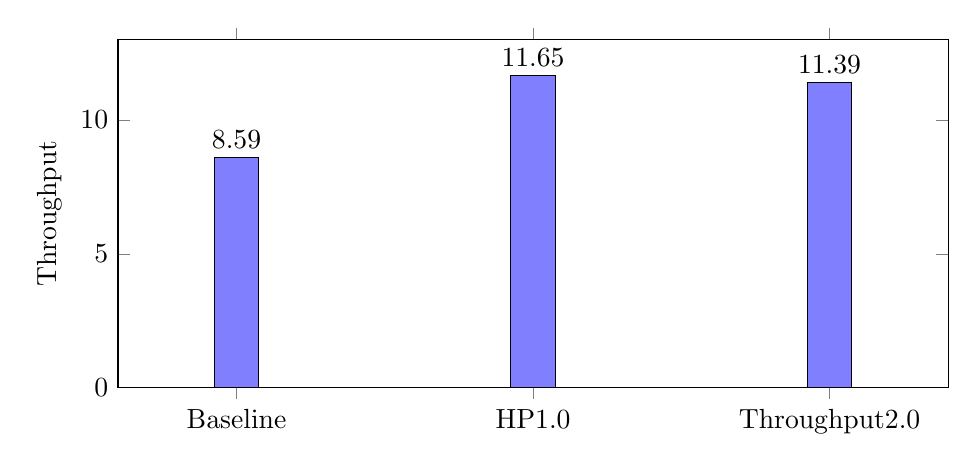
\begin{tikzpicture}
\begin{axis}[
    ybar,
    bar width=16pt,
    width=\textwidth,
    height=6cm,
    ymin=0,
    ymax=13,
    ylabel={Throughput},
    symbolic x coords={Baseline,HP1.0,Throughput2.0},
    xtick=data,
    nodes near coords,
    nodes near coords align={vertical},
    enlarge x limits=0.2
]
\addplot[fill=blue!50] coordinates {
(Baseline,8.587)
(HP1.0,11.654)
(Throughput2.0,11.388)
};
\end{axis}
\end{tikzpicture}
\caption{High-load throughput.}
\end{subfigure}
\hfill
\begin{subfigure}[t]{0.48\textwidth}
\centering
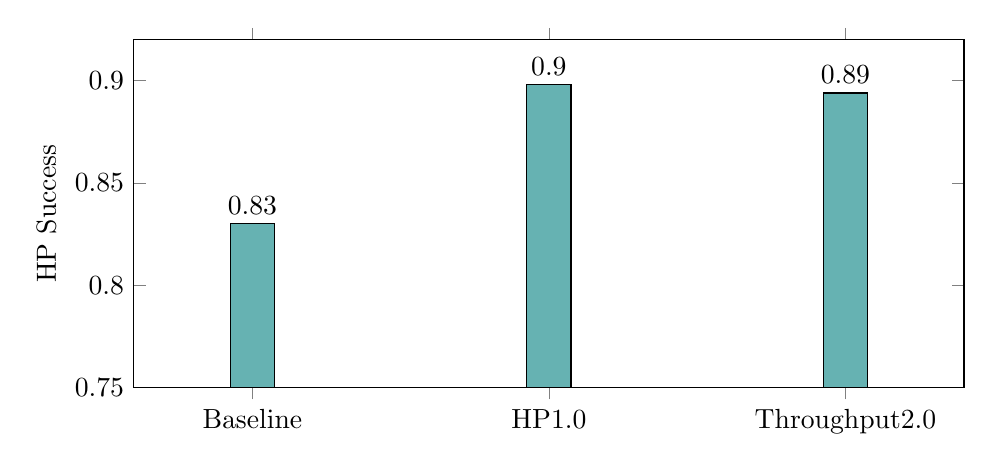
\begin{tikzpicture}
\begin{axis}[
    ybar,
    bar width=16pt,
    width=\textwidth,
    height=6cm,
    ymin=0.75,
    ymax=0.92,
    ylabel={HP Success},
    symbolic x coords={Baseline,HP1.0,Throughput2.0},
    xtick=data,
    nodes near coords,
    nodes near coords align={vertical},
    enlarge x limits=0.2
]
\addplot[fill=teal!60] coordinates {
(Baseline,0.830)
(HP1.0,0.898)
(Throughput2.0,0.894)
};
\end{axis}
\end{tikzpicture}
\caption{High-load high-priority success rate.}
\end{subfigure}
\caption{Count-based reward ablation on the high-load scenario. Lowering the high-priority penalty fixes the over-conservative regime; increasing throughput weight maximizes scalar reward but produces a different trade-off.}
\label{fig:count_ablation_bars}
\end{figure}

\begin{figure}[H]
\centering
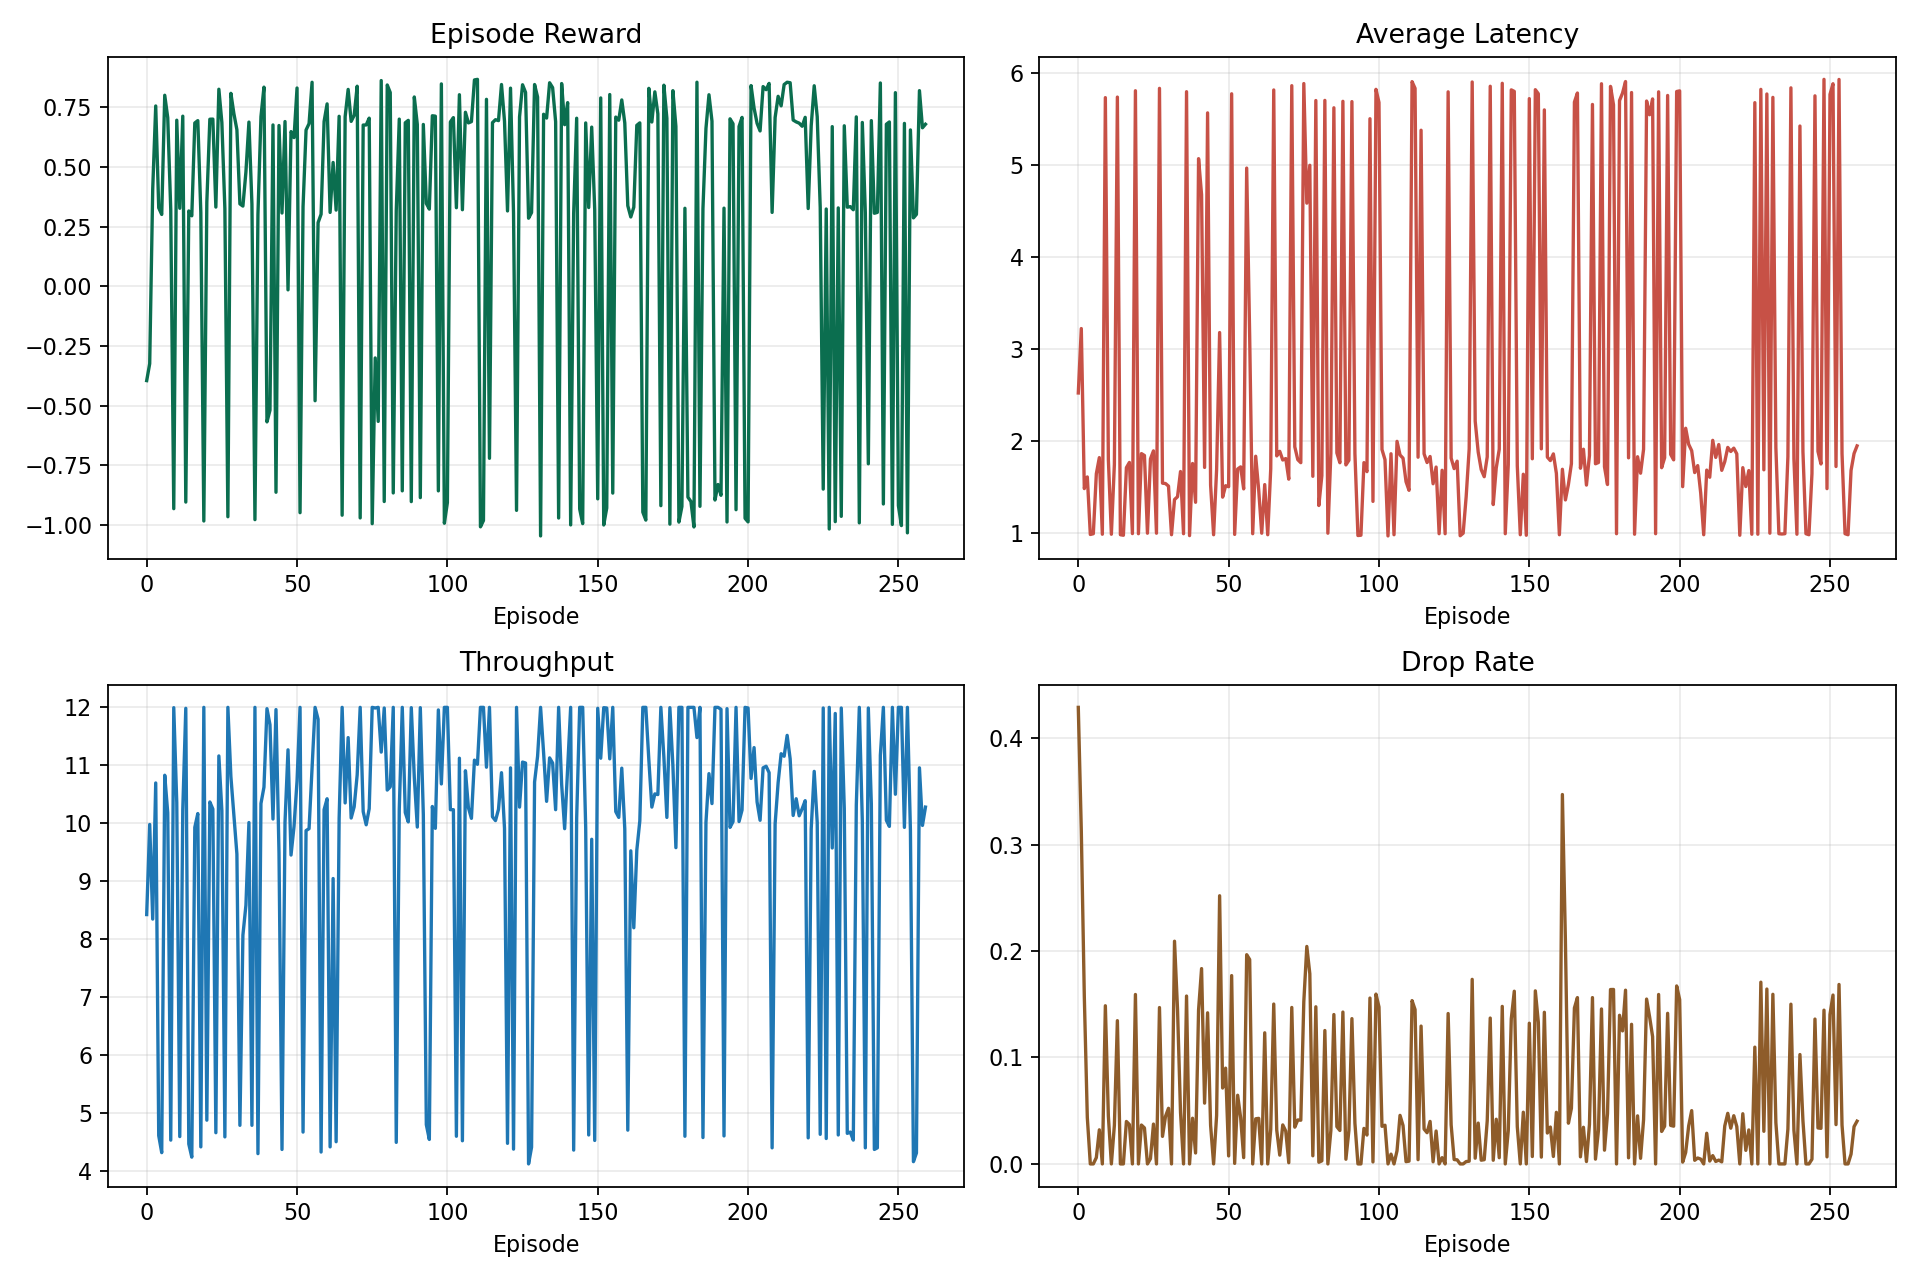
\includegraphics[width=0.9\textwidth]{count_training_curves.png}
\caption{Representative count-based PPO training curves. Reward and core operating metrics stabilize after early improvement, showing that the count-based setting is comparatively easy to optimize once the reward weights are sensible.}
\label{fig:count_training_curves}
\end{figure}

\begin{figure}[H]
\centering
\begin{subfigure}[t]{0.48\textwidth}
\centering
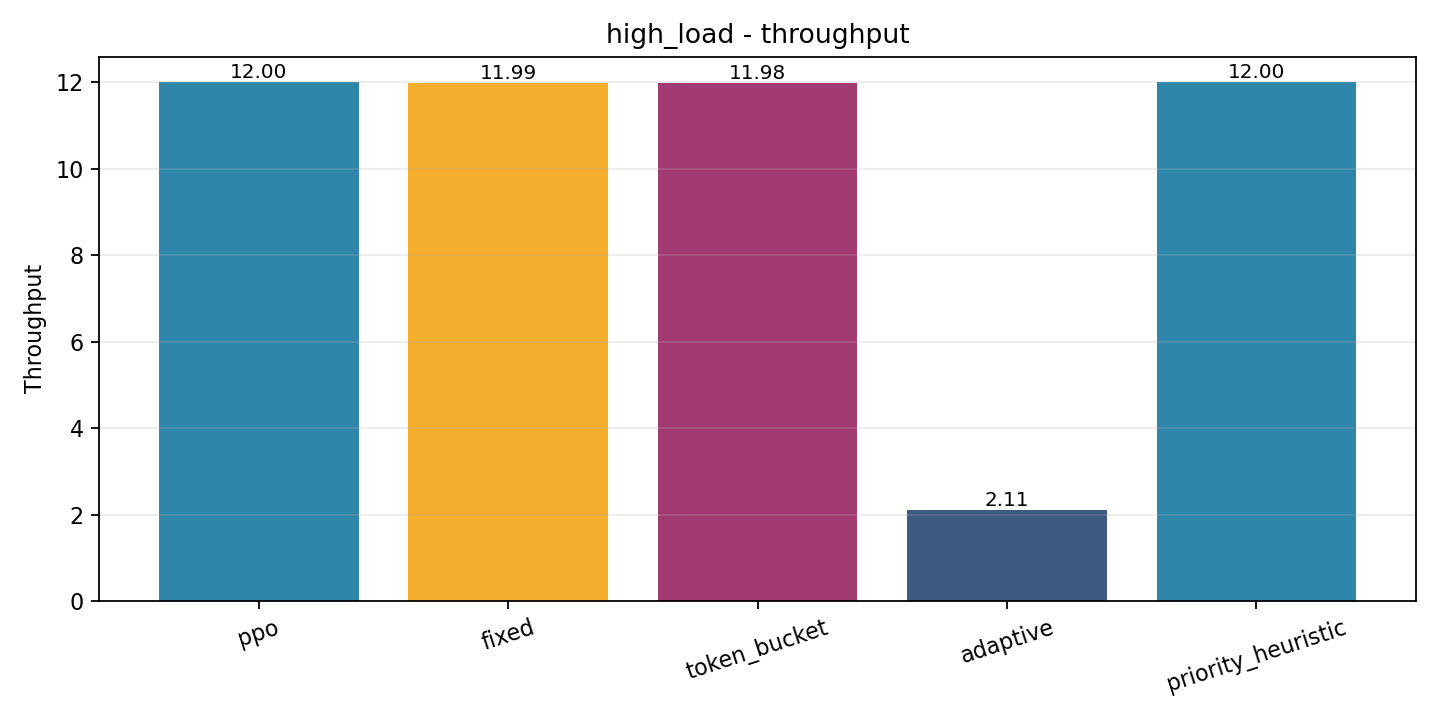
\includegraphics[width=\textwidth]{count_high_load_throughput.png}
\caption{High-load throughput comparison.}
\end{subfigure}
\hfill
\begin{subfigure}[t]{0.48\textwidth}
\centering
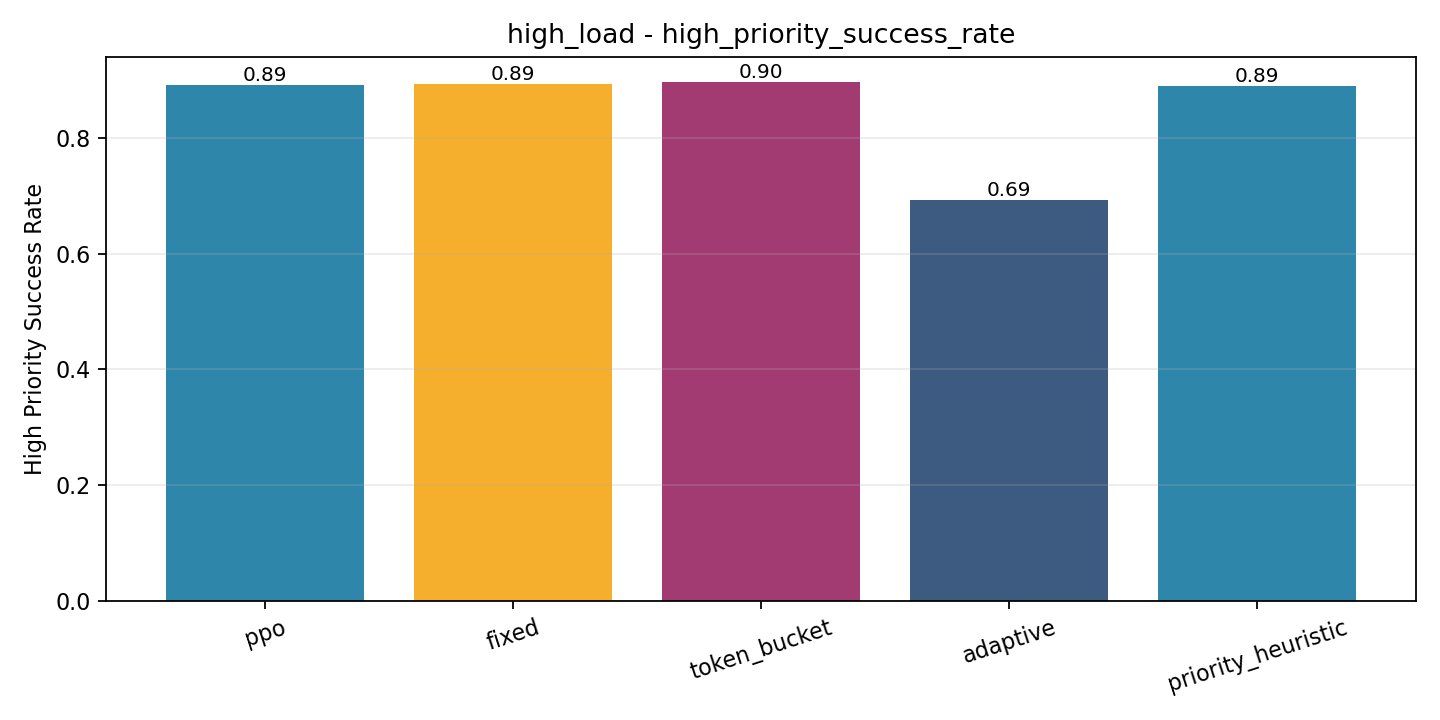
\includegraphics[width=\textwidth]{count_high_load_hp_success.png}
\caption{High-load high-priority success comparison.}
\end{subfigure}
\caption{Count-based high-load plots from the final evaluation pipeline. These emphasize that PPO can be highly competitive once the high-priority penalty is no longer overly conservative.}
\label{fig:count_high_load_real_plots}
\end{figure}

\subsection{Cost-Aware Extension: Naive Reward Failure}
The first cost-aware reward design failed. The environment now constrained service by cost budget, but the reward still treated raw request count as the main positive outcome. The agent eventually learned a degenerate policy that mostly chose \texttt{decrease}, admitted very little traffic, and left much of the useful budget under-exploited.

Table~\ref{tab:naive_cost_failure} shows the final policy under that naive reward. Throughput is catastrophic, budget utilization is low, and drop rates are extremely high. The lesson is that merely adding a cost bonus is not enough if the dominant optimization target is still misaligned with the environment.

\begin{table}[H]
\centering
\caption{Final behavior of the naive cost-aware PPO after collapse. The agent under-serves badly and does not use the budget effectively.}
\label{tab:naive_cost_failure}
\resizebox{\textwidth}{!}{
\begin{tabular}{lcccccc}
\toprule
Scenario & Reward & Throughput & Latency & Drop Rate & HP Success & Budget Util. \\
\midrule
low\_load & $-90.697$ & $1.987$ & $1.332$ & $0.494$ & $0.487$ & $0.247$ \\
high\_load & $-238.482$ & $2.111$ & $2.033$ & $0.870$ & $0.707$ & $0.265$ \\
bursty & $-193.098$ & $2.109$ & $1.882$ & $0.787$ & $0.674$ & $0.264$ \\
oscillating & $-197.505$ & $2.107$ & $1.822$ & $0.813$ & $0.706$ & $0.265$ \\
\bottomrule
\end{tabular}
}
\end{table}

The collapse is visible in Figure~\ref{fig:collapse_curve}. The policy reached a reasonable region, then diverged into a pathological low-admission strategy after roughly episode $180$.

\begin{figure}[H]
\centering
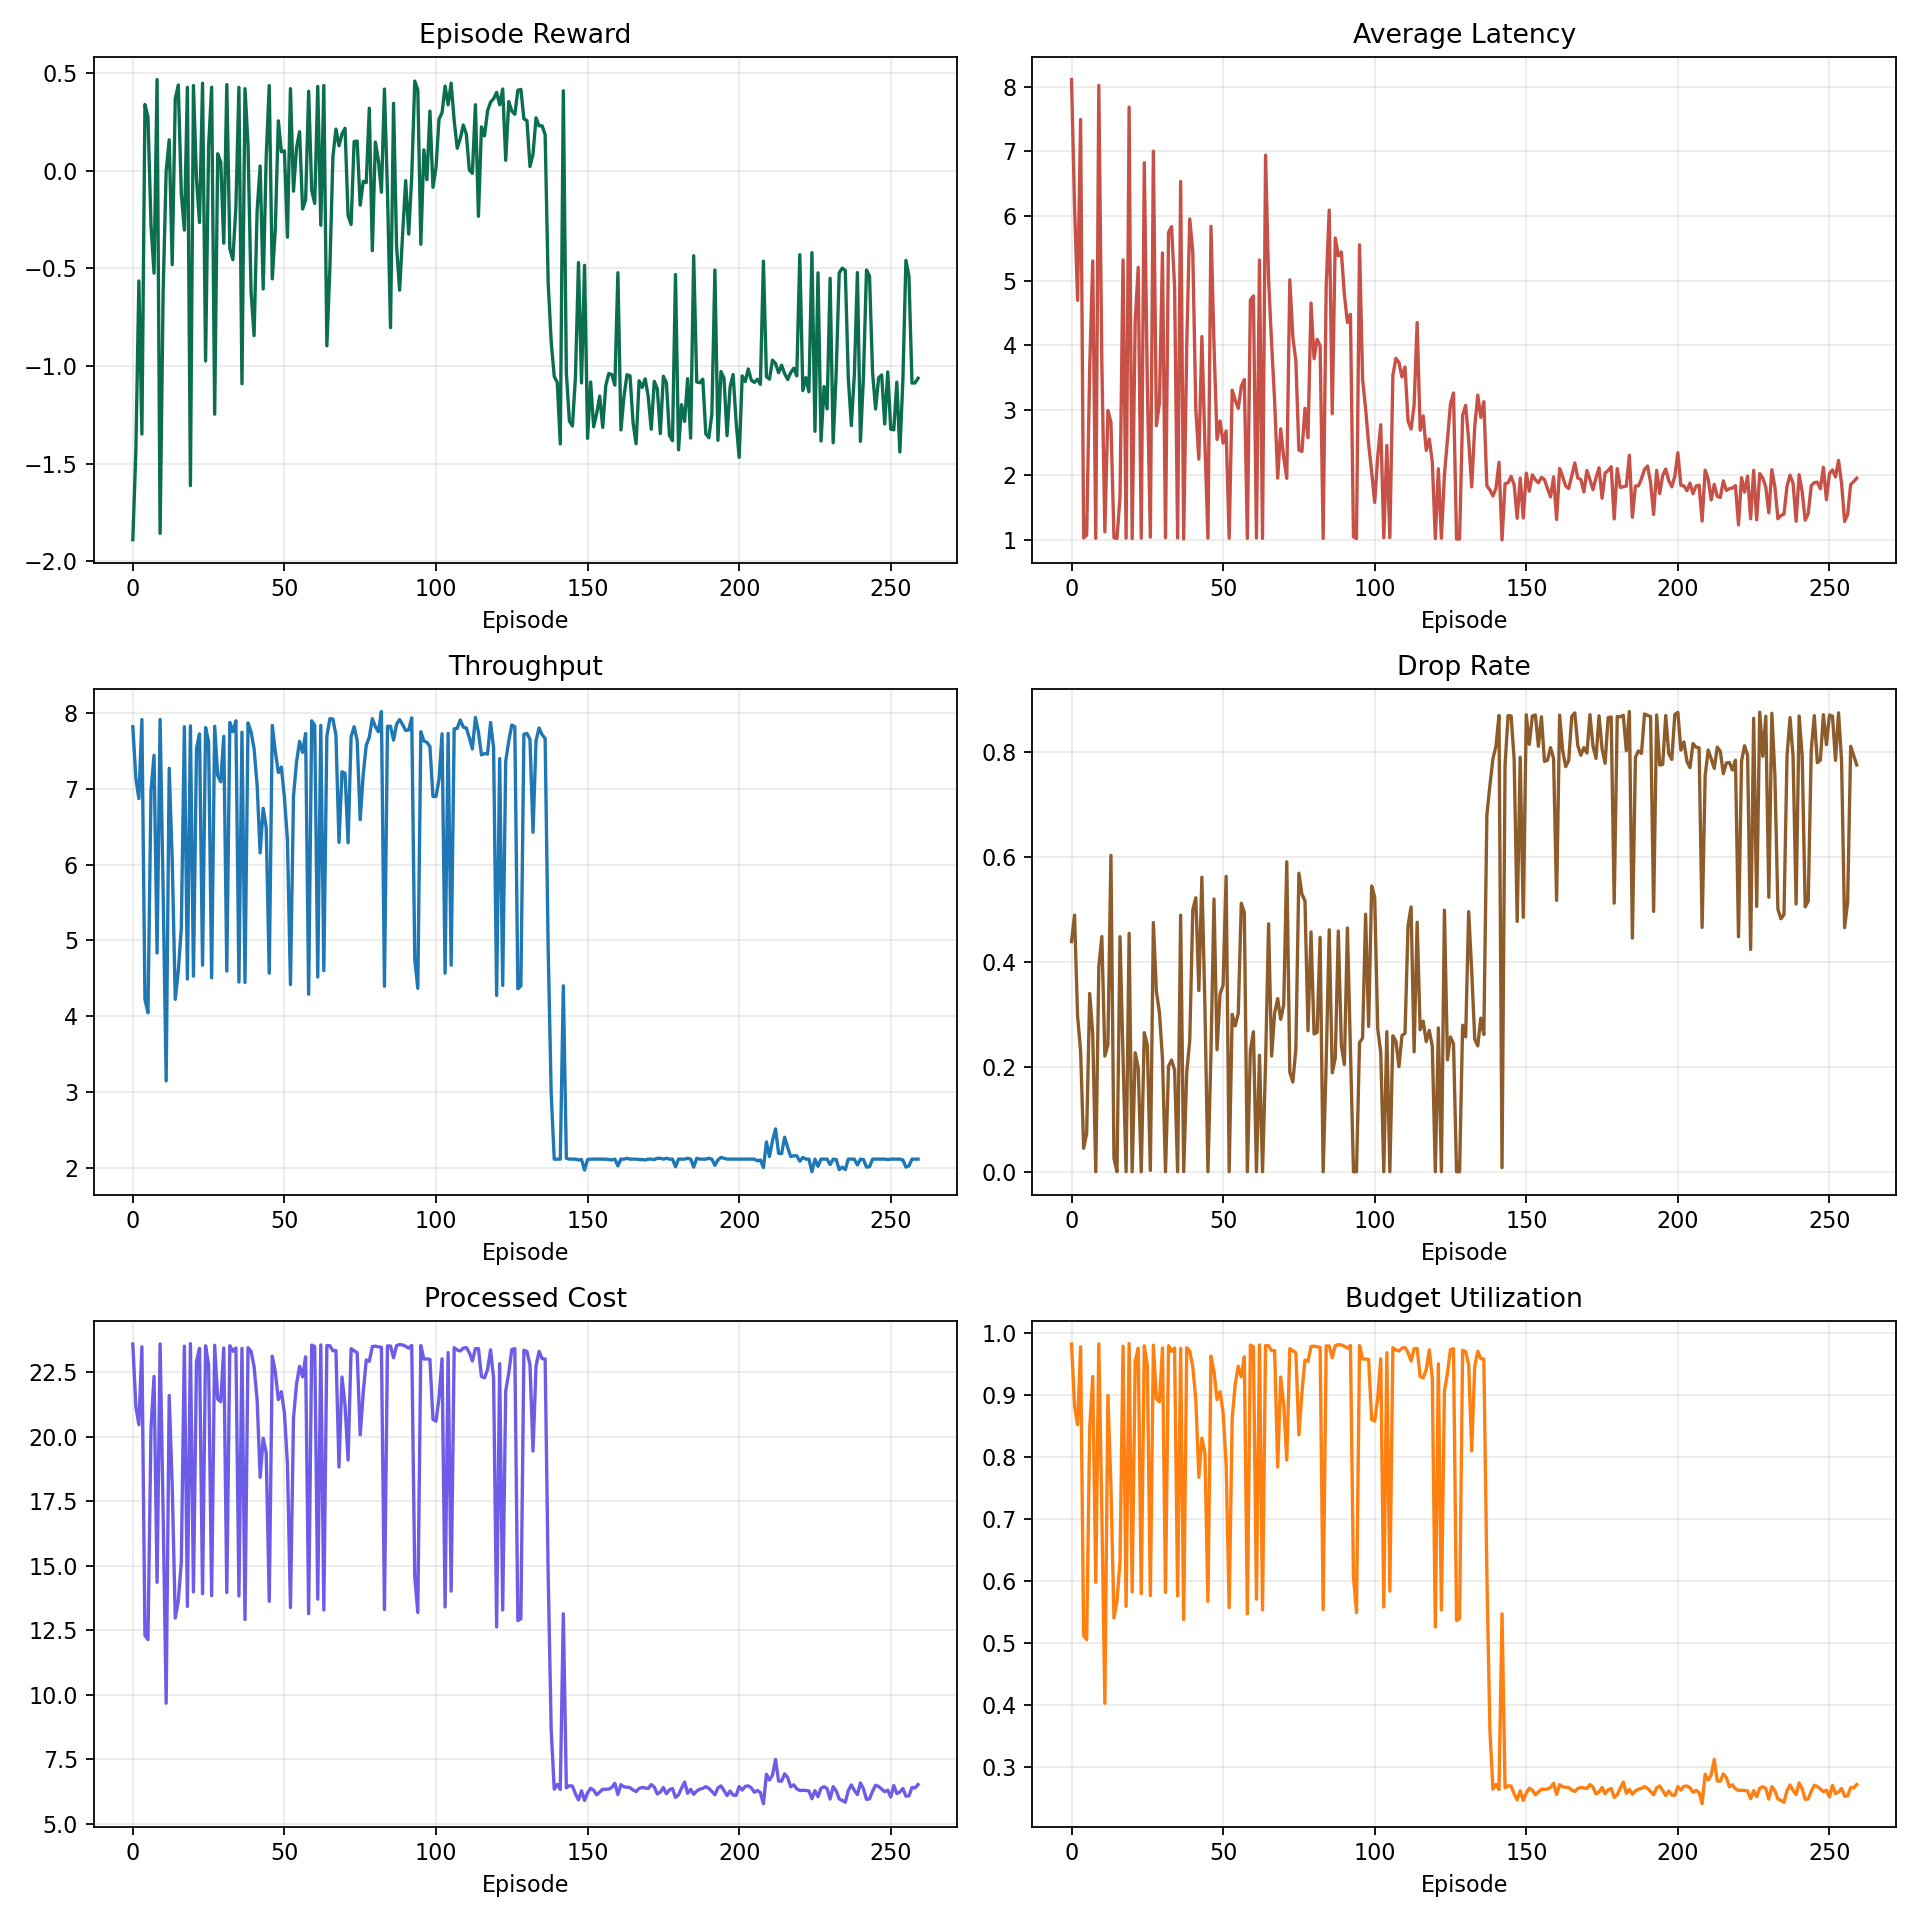
\includegraphics[width=0.9\textwidth]{naive_cost_training_curves.png}
\caption{Training curves for the naive cost-aware PPO. After a promising mid-training phase, reward and throughput collapse while the agent drifts toward a near-always-decrease policy.}
\label{fig:collapse_curve}
\end{figure}

\subsection{Cost-Only Reward vs. Count-Blind PPO}
The key recovery step was to replace request-count throughput with processed cost. Table~\ref{tab:cost_vs_blind} compares the selected count-blind PPO used in later experiments (\texttt{cost\_blind\_hp15}) against the final cost-aware \texttt{cost\_only} PPO.

\begin{table}[H]
\centering
\caption{Count-blind versus cost-aware PPO. The cost-aware policy trades raw request throughput for high served cost and very high budget utilization. OOD cost-shift scenarios apply only to the cost-aware setting.}
\label{tab:cost_vs_blind}
\resizebox{\textwidth}{!}{
\begin{tabular}{llcccccc}
\toprule
Scenario & Policy & Reward & Throughput & Latency & Drop Rate & HP Success & Budget Util. \\
\midrule
\multirow{2}{*}{low\_load}
& PPO-CountBlind-HP1.5 & $57.598$ & $4.508$ & $0.987$ & $0.000$ & $0.482$ & $0.376$ \\
& PPO-CostOnly & $133.114$ & $4.479$ & $1.020$ & $0.000$ & $0.491$ & $0.557$ \\
\midrule
\multirow{2}{*}{high\_load}
& PPO-CountBlind-HP1.5 & $-173.772$ & $11.998$ & $5.805$ & $0.150$ & $0.892$ & $1.000$ \\
& PPO-CostOnly & $102.018$ & $7.800$ & $3.227$ & $0.479$ & $0.882$ & $0.975$ \\
\midrule
\multirow{2}{*}{bursty}
& PPO-CountBlind-HP1.5 & $124.530$ & $10.134$ & $1.821$ & $0.033$ & $0.739$ & $0.844$ \\
& PPO-CostOnly & $164.421$ & $7.744$ & $2.836$ & $0.199$ & $0.752$ & $0.966$ \\
\midrule
\multirow{2}{*}{oscillating}
& PPO-CountBlind-HP1.5 & $145.492$ & $10.881$ & $1.692$ & $0.004$ & $0.801$ & $0.907$ \\
& PPO-CostOnly & $157.797$ & $7.799$ & $2.901$ & $0.258$ & $0.802$ & $0.975$ \\
\midrule
cheap\_flood & PPO-CostOnly & $171.282$ & $15.660$ & $1.090$ & $0.086$ & $0.575$ & $0.772$ \\
expensive\_attack & PPO-CostOnly & $-1203.074$ & $1.704$ & $39.380$ & $0.893$ & $0.125$ & $0.850$ \\
mixed\_shift & PPO-CostOnly & $-731.946$ & $2.767$ & $24.412$ & $0.791$ & $0.769$ & $0.948$ \\
\bottomrule
\end{tabular}
}
\end{table}

The standard scenarios reveal a deliberate trade-off. The count-blind agent serves more requests, but the cost-aware agent uses the cost budget much more consistently and improves reward substantially on \texttt{high\_load}. The OOD results are mixed: \texttt{cheap\_flood} is handled well, while \texttt{expensive\_attack} remains a major failure mode.

\begin{figure}[H]
\centering
\begin{subfigure}[t]{0.48\textwidth}
\centering
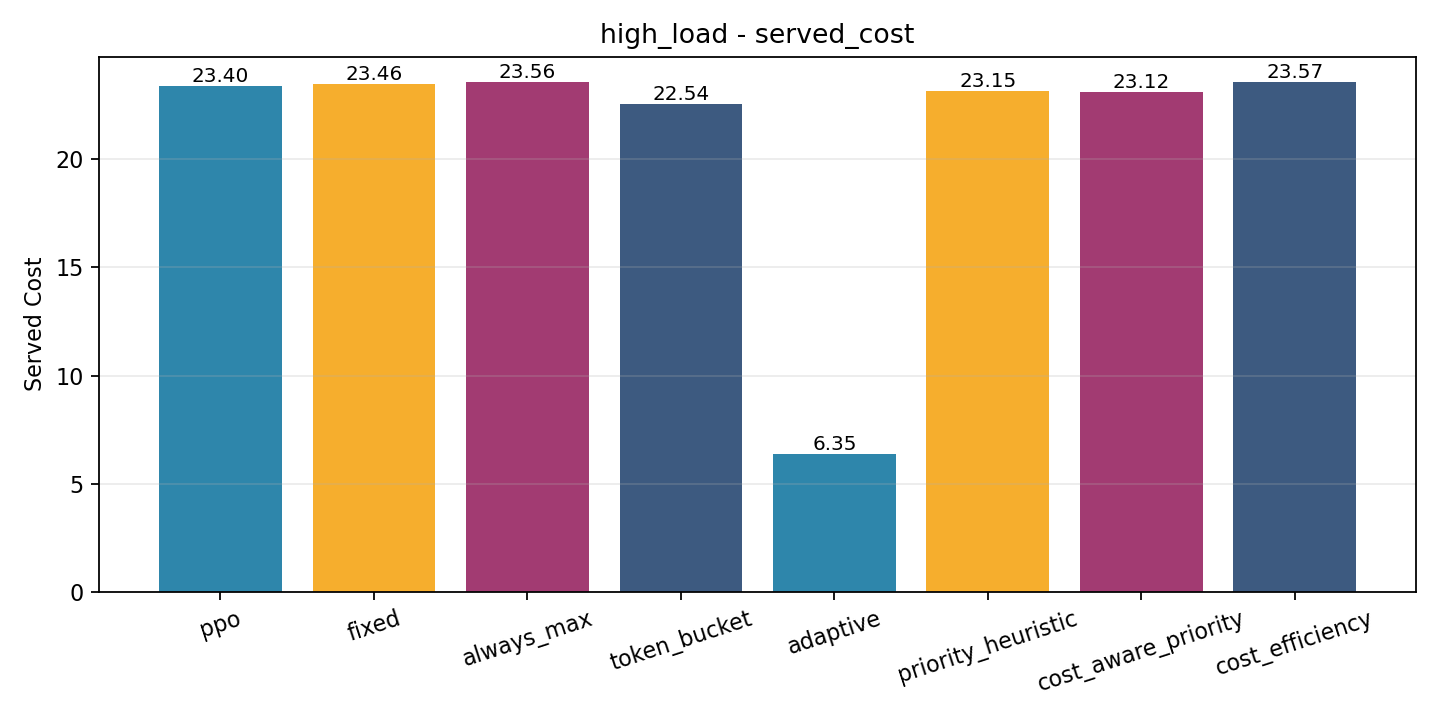
\includegraphics[width=\textwidth]{cost_high_load_served_cost.png}
\caption{High-load served cost.}
\end{subfigure}
\hfill
\begin{subfigure}[t]{0.48\textwidth}
\centering
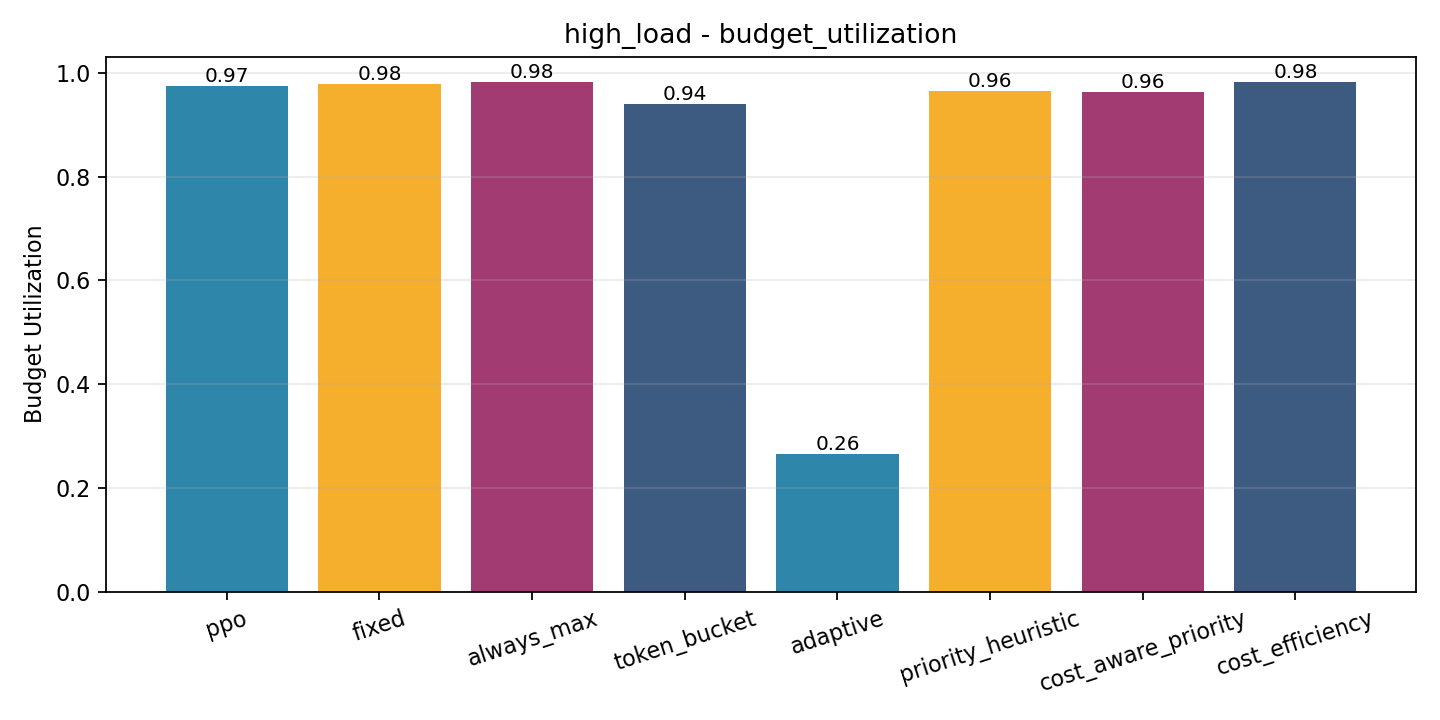
\includegraphics[width=\textwidth]{cost_high_load_budget_utilization.png}
\caption{High-load budget utilization.}
\end{subfigure}
\caption{Cost-only PPO under high-load. The learned agent saturates the budget and keeps served computational work high even though raw request throughput is lower than in the count-blind setting.}
\label{fig:cost_high_load_cost_metrics}
\end{figure}

\begin{figure}[H]
\centering
\begin{subfigure}[t]{0.48\textwidth}
\centering
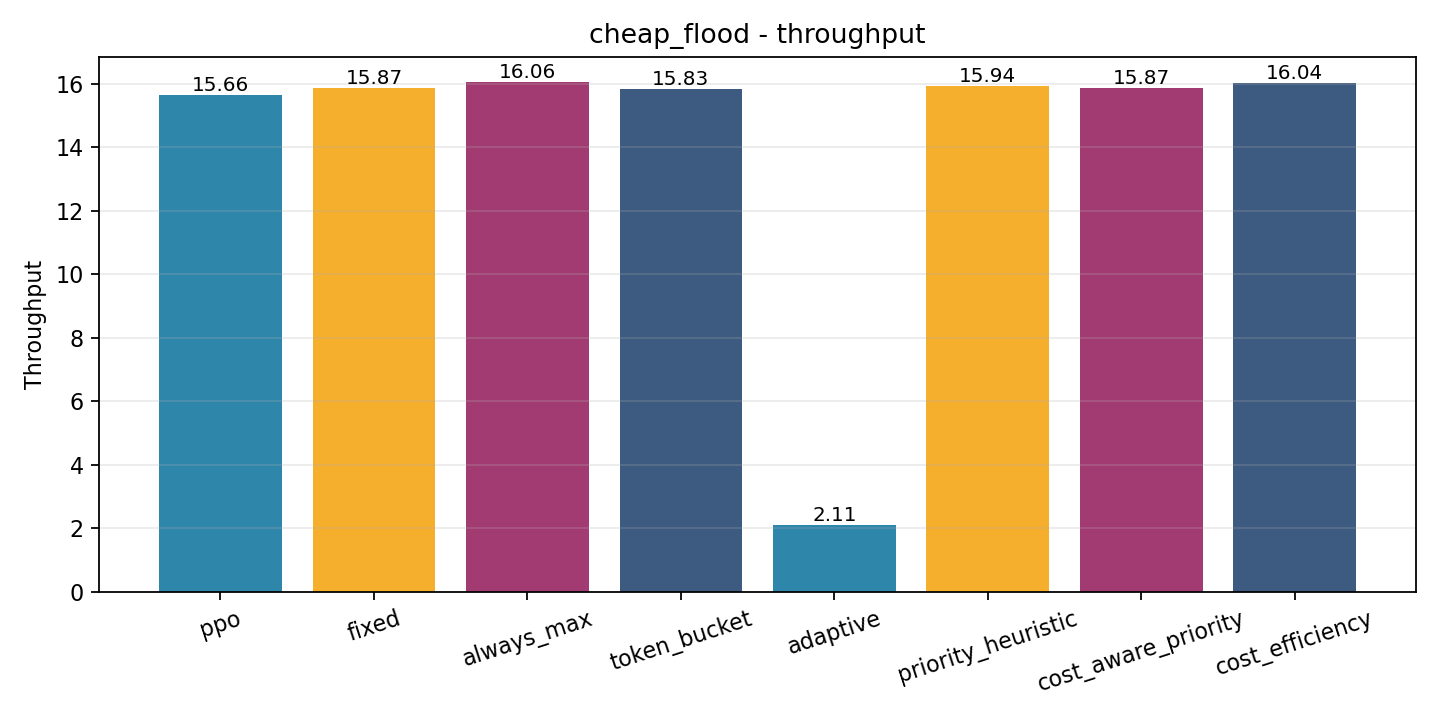
\includegraphics[width=\textwidth]{cost_cheap_flood_throughput.png}
\caption{Cheap-flood throughput.}
\end{subfigure}
\hfill
\begin{subfigure}[t]{0.48\textwidth}
\centering
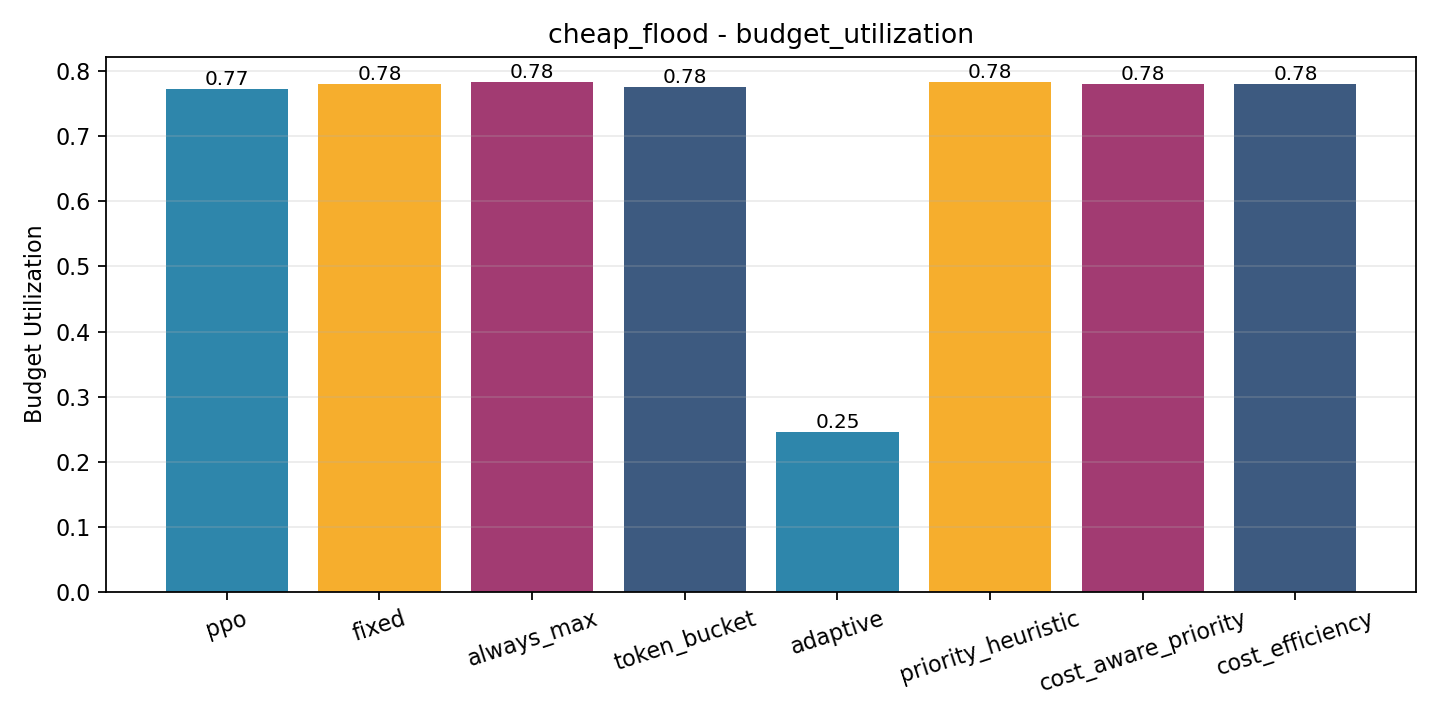
\includegraphics[width=\textwidth]{cost_cheap_flood_budget_utilization.png}
\caption{Cheap-flood budget utilization.}
\end{subfigure}
\caption{OOD cheap-flood scenario. The cost-aware PPO generalizes well when many low-cost requests can be packed efficiently into the available budget.}
\label{fig:cheap_flood_ood}
\end{figure}

\begin{figure}[H]
\centering
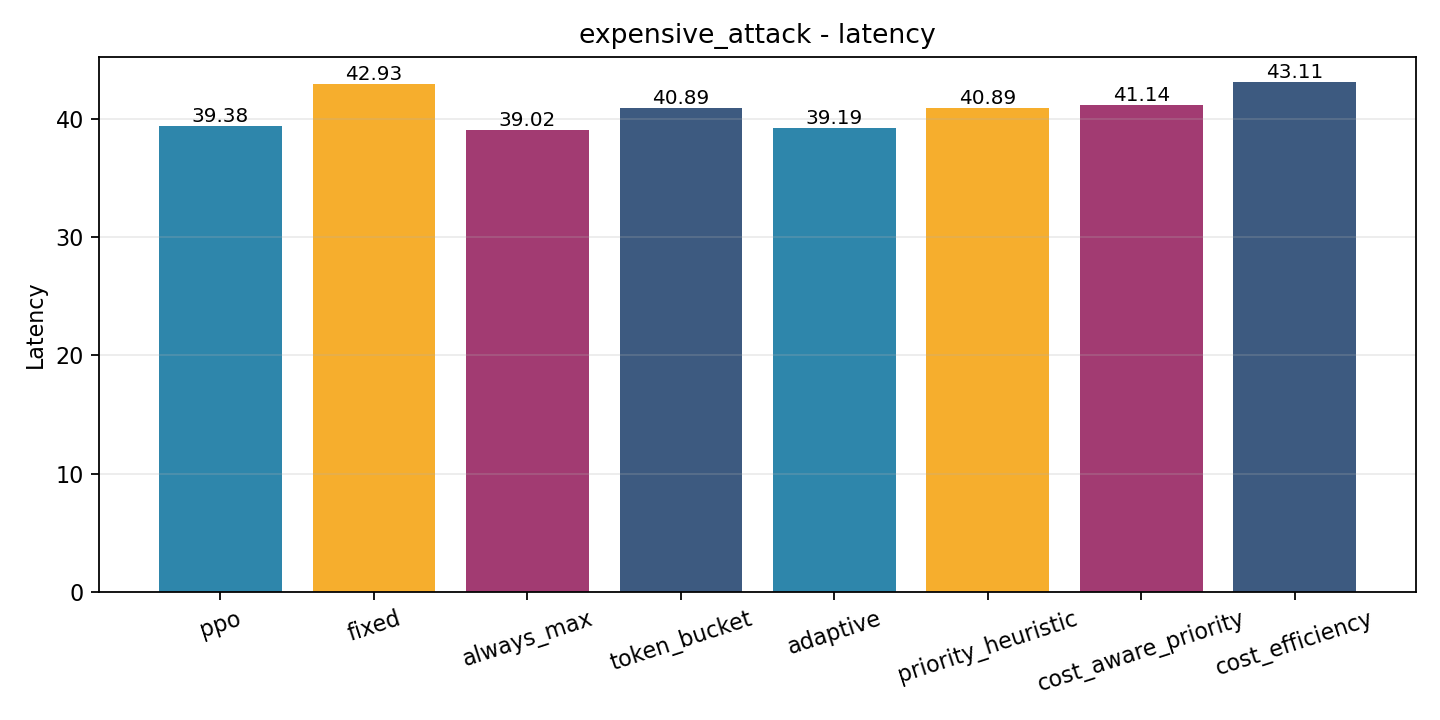
\includegraphics[width=0.78\textwidth]{cost_expensive_attack_latency.png}
\caption{OOD expensive-attack scenario. Latency explodes because a few high-cost requests dominate the budget, exposing a major generalization weakness of the cost-aware PPO.}
\label{fig:expensive_attack_latency}
\end{figure}

\subsection{Comparison with Cost-Aware Heuristics}
The next question is whether cost-aware PPO can outperform cost-aware heuristics that explicitly exploit domain structure. Table~\ref{tab:heuristic_compare} focuses on the most informative scenarios. The answer is mixed: PPO is competitive, but not dominant.

\begin{table}[H]
\centering
\caption{Cost-aware PPO compared with strong cost-aware heuristics. PPO remains competitive, but the best heuristics still win on several stress scenarios.}
\label{tab:heuristic_compare}
\resizebox{\textwidth}{!}{
\begin{tabular}{llccccc}
\toprule
Scenario & Policy & Reward & Throughput & Latency & Drop Rate & HP Success \\
\midrule
\multirow{5}{*}{high\_load}
& PPO-CostOnly & $102.018$ & $7.800$ & $3.227$ & $0.479$ & $0.882$ \\
& Fixed-Cost & $58.704$ & $7.882$ & $4.154$ & $0.460$ & $0.893$ \\
& TokenBucket-Cost & $117.727$ & $7.502$ & $1.617$ & $0.500$ & $0.896$ \\
& PriorityHeuristic-Cost & $119.645$ & $7.725$ & $2.121$ & $0.484$ & $0.892$ \\
& CostAwarePriority & $120.169$ & $7.687$ & $2.067$ & $0.484$ & $0.892$ \\
\midrule
\multirow{5}{*}{bursty}
& PPO-CostOnly & $164.421$ & $7.744$ & $2.836$ & $0.199$ & $0.752$ \\
& Fixed-Cost & $165.857$ & $7.205$ & $1.547$ & $0.234$ & $0.744$ \\
& TokenBucket-Cost & $153.565$ & $6.946$ & $1.364$ & $0.265$ & $0.747$ \\
& PriorityHeuristic-Cost & $167.142$ & $7.271$ & $1.547$ & $0.237$ & $0.745$ \\
& CostAwarePriority & $162.773$ & $7.139$ & $1.483$ & $0.242$ & $0.765$ \\
\midrule
\multirow{5}{*}{oscillating}
& PPO-CostOnly & $157.797$ & $7.799$ & $2.901$ & $0.258$ & $0.802$ \\
& Fixed-Cost & $164.414$ & $7.656$ & $2.069$ & $0.272$ & $0.806$ \\
& TokenBucket-Cost & $156.464$ & $7.328$ & $1.388$ & $0.308$ & $0.806$ \\
& PriorityHeuristic-Cost & $167.337$ & $7.587$ & $1.708$ & $0.277$ & $0.800$ \\
& CostAwarePriority & $165.515$ & $7.564$ & $1.709$ & $0.283$ & $0.800$ \\
\midrule
\multirow{5}{*}{expensive\_attack}
& PPO-CostOnly & $-1203.074$ & $1.704$ & $39.380$ & $0.893$ & $0.125$ \\
& Fixed-Cost & $-1260.292$ & $1.640$ & $42.931$ & $0.926$ & $0.074$ \\
& TokenBucket-Cost & $-1199.342$ & $1.637$ & $40.890$ & $0.927$ & $0.074$ \\
& PriorityHeuristic-Cost & $-1199.342$ & $1.637$ & $40.890$ & $0.927$ & $0.074$ \\
& CostAwarePriority & $-1204.929$ & $1.631$ & $41.144$ & $0.927$ & $0.073$ \\
\bottomrule
\end{tabular}
}
\end{table}

A useful summary is the scenario-level winner by total reward:
\begin{itemize}[leftmargin=1.5em]
    \item \textbf{high\_load}: CostAwarePriority
    \item \textbf{bursty}: PriorityHeuristic-Cost
    \item \textbf{oscillating}: PriorityHeuristic-Cost
    \item \textbf{cheap\_flood}: AlwaysMax
    \item \textbf{expensive\_attack}: AlwaysMax (least negative)
    \item \textbf{mixed\_shift}: AlwaysMax (least negative)
\end{itemize}

This ranking reinforces the central conclusion: PPO learns meaningful cost-aware behavior, but strong heuristics remain formidable.

\begin{figure}[H]
\centering
\begin{subfigure}[t]{0.48\textwidth}
\centering
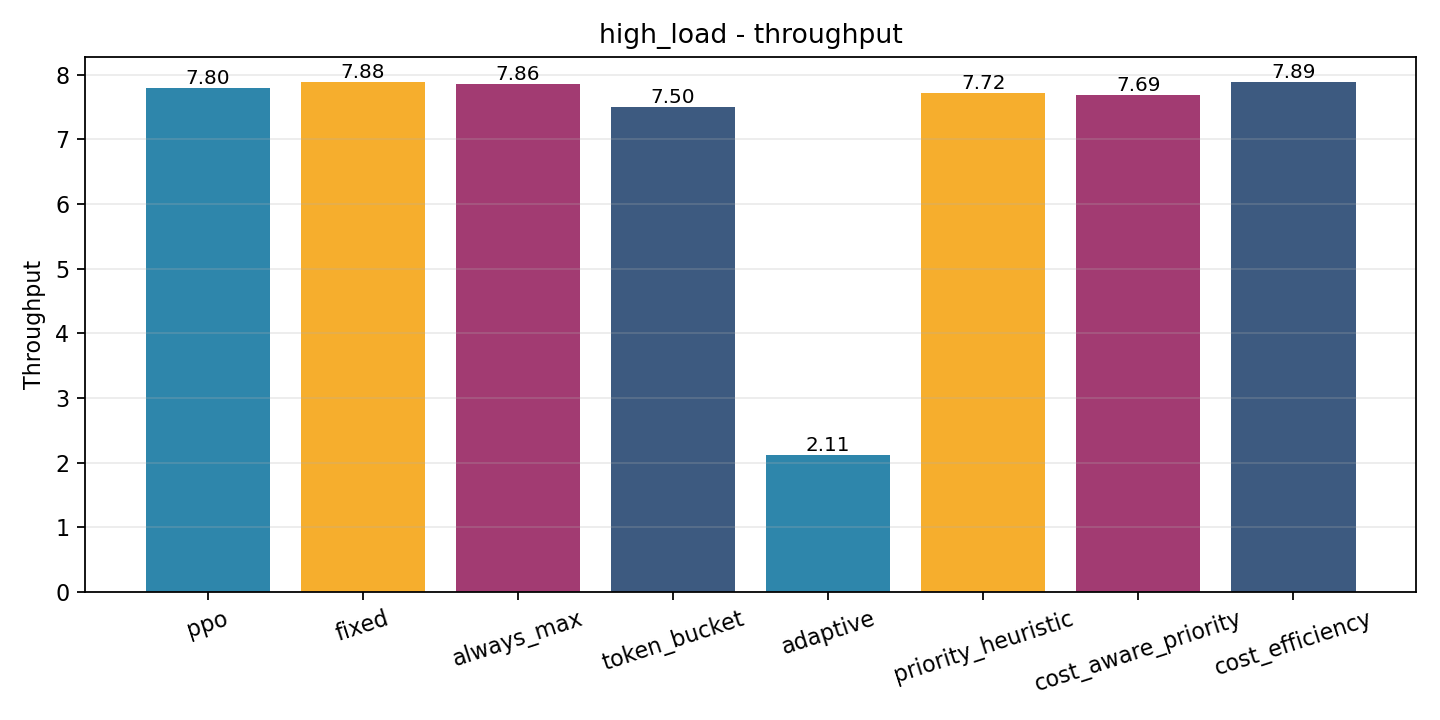
\includegraphics[width=\textwidth]{cost_high_load_throughput.png}
\caption{High-load throughput across PPO and heuristics.}
\end{subfigure}
\hfill
\begin{subfigure}[t]{0.48\textwidth}
\centering
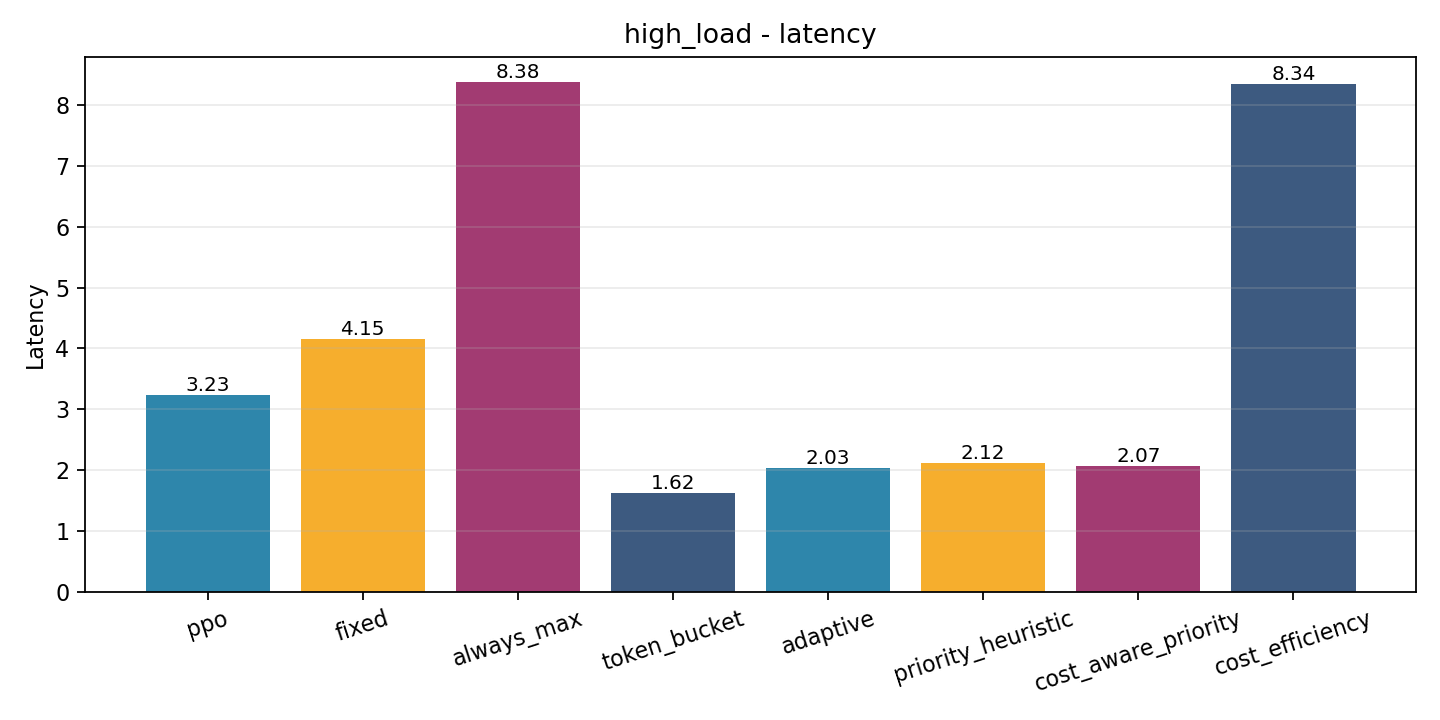
\includegraphics[width=\textwidth]{cost_high_load_latency.png}
\caption{High-load latency across PPO and heuristics.}
\end{subfigure}
\caption{Cost-aware high-load comparison. PPO remains competitive, but the strongest heuristics achieve better latency-reward trade-offs in the most difficult in-distribution scenario.}
\label{fig:cost_high_load_heuristics}
\end{figure}

\subsection{Fine-Tuning Attempt}
The final experiment asked whether a short specialization stage on \texttt{high\_load} could push cost-aware PPO above the heuristics. Table~\ref{tab:finetune} shows the answer.

\begin{table}[H]
\centering
\caption{High-load fine-tuning of the cost-aware PPO. The specialized agent improves slightly on the target scenario but still does not surpass the strongest heuristics, and it hurts OOD performance on \texttt{expensive\_attack}.}
\label{tab:finetune}
\resizebox{\textwidth}{!}{
\begin{tabular}{lcccccc}
\toprule
Setting & Scenario & Reward & Throughput & Latency & Drop Rate & HP Success \\
\midrule
\multirow{4}{*}{Base PPO-CostOnly}
& high\_load & $102.018$ & $7.800$ & $3.227$ & $0.479$ & $0.882$ \\
& bursty & $164.421$ & $7.744$ & $2.836$ & $0.199$ & $0.752$ \\
& oscillating & $157.797$ & $7.799$ & $2.901$ & $0.258$ & $0.802$ \\
& expensive\_attack & $-1203.074$ & $1.704$ & $39.380$ & $0.893$ & $0.125$ \\
\midrule
\multirow{4}{*}{High-Load Fine-Tuned PPO}
& high\_load & $106.937$ & $7.808$ & $3.176$ & $0.471$ & $0.886$ \\
& bursty & $161.071$ & $7.724$ & $2.919$ & $0.205$ & $0.746$ \\
& oscillating & $155.723$ & $7.841$ & $3.121$ & $0.252$ & $0.795$ \\
& expensive\_attack & $-1219.551$ & $1.645$ & $41.595$ & $0.926$ & $0.074$ \\
\bottomrule
\end{tabular}
}
\end{table}

The specialization improved the in-distribution target slightly, but it did not beat the best heuristic on \texttt{high\_load}, and it noticeably degraded robustness to the expensive OOD attack. This suggests that the main limitation is not just under-training but a deeper mismatch between the learned policy and the unseen cost distribution.

\subsection{Warm-Started PPO from Heuristic Demonstrations}
The final novelty experiment asked whether PPO could be safely warm-started from a strong heuristic and then improved with reinforcement learning. A demonstration dataset of $54{,}000$ state-action pairs was collected from the \texttt{cost\_aware\_priority} heuristic across the standard traffic scenarios. Behavioral cloning produced a teacher-like policy with validation accuracy around $0.53$, which was sufficient to nearly match the heuristic on some scenarios.

However, naive PPO fine-tuning from the cloned checkpoint collapsed. The learned policy drifted away from the teacher and converged to a poor high-latency regime. To prevent this, a behavior-regularized PPO objective was introduced. The PPO actor update was augmented with a teacher-action anchoring term:
\begin{equation}
\mathcal{L}_{\text{reg}} = \mathcal{L}_{\text{PPO}} - \lambda \, \mathbb{E}\left[\log \pi_\theta(a^{\text{teacher}} \mid s)\right].
\end{equation}
This term encourages the policy to stay close to the safe teacher behavior while still optimizing reward.

Table~\ref{tab:warmstart} shows the final result for the full $\lambda=0.1$ run, which was the best stable setting. The cloned policy already transferred much of the heuristic behavior. Behavior-regularized fine-tuning prevented catastrophic collapse and improved the cloned policy on bursty, oscillating, and low-load scenarios, although it still did not surpass the teacher overall.

\begin{table}[H]
\centering
\caption{Warm-started PPO from heuristic demonstrations. Behavioral cloning successfully transfers teacher behavior; behavior-regularized PPO with $\lambda=0.1$ prevents collapse and gives modest gains over the cloned policy, but still trails the teacher on the main stress scenarios.}
\label{tab:warmstart}
\resizebox{\textwidth}{!}{
\begin{tabular}{llccccc}
\toprule
Scenario & Policy & Reward & Throughput & Latency & Drop Rate & HP Success \\
\midrule
\multirow{3}{*}{high\_load}
& Teacher: CostAwarePriority & $120.169$ & $7.687$ & $2.067$ & $0.484$ & $0.892$ \\
& PPO-Cloned & $108.240$ & $7.326$ & $1.583$ & $0.516$ & $0.897$ \\
& PPO-Regularized ($\lambda=0.1$) & $105.752$ & $7.232$ & $1.521$ & $0.520$ & $0.893$ \\
\midrule
\multirow{3}{*}{bursty}
& Teacher: CostAwarePriority & $162.773$ & $7.139$ & $1.483$ & $0.242$ & $0.765$ \\
& PPO-Cloned & $142.419$ & $7.376$ & $2.477$ & $0.273$ & $0.750$ \\
& PPO-Regularized ($\lambda=0.1$) & $152.224$ & $7.716$ & $2.994$ & $0.217$ & $0.741$ \\
\midrule
\multirow{3}{*}{oscillating}
& Teacher: CostAwarePriority & $165.515$ & $7.564$ & $1.709$ & $0.283$ & $0.800$ \\
& PPO-Cloned & $160.913$ & $7.459$ & $1.651$ & $0.288$ & $0.795$ \\
& PPO-Regularized ($\lambda=0.1$) & $162.030$ & $7.623$ & $2.073$ & $0.273$ & $0.802$ \\
\midrule
\multirow{3}{*}{low\_load}
& Teacher: CostAwarePriority & $127.468$ & $4.354$ & $1.013$ & $0.012$ & $0.488$ \\
& PPO-Cloned & $129.053$ & $4.398$ & $1.015$ & $0.010$ & $0.481$ \\
& PPO-Regularized ($\lambda=0.1$) & $131.856$ & $4.447$ & $1.018$ & $0.001$ & $0.491$ \\
\bottomrule
\end{tabular}
}
\end{table}

Two additional quick screens tested stronger anchors, $\lambda=0.15$ and $\lambda=0.2$. Neither improved the target \texttt{high\_load} scenario, and both performed worse than the full $\lambda=0.1$ run. This suggests that moderate regularization is necessary: too weak an anchor allows destructive drift, but too strong an anchor over-constrains learning and prevents useful adaptation.

\subsection{Azure-Calibrated Cost Transfer}
The final transfer-learning experiment replaced the synthetic request-cost distribution with one derived from the public Azure Functions Invocation Trace 2021. The trace contains approximately $1.81$ million invocation records. A random sample of $500{,}000$ durations was used to estimate the cost profile. The median duration was $0.046$ seconds and the empirical $95$th percentile was $18.845$ seconds. After scaling the median to simulator cost $3$ and clipping at cost $15$, the resulting PMF was highly bimodal, with $40.9\%$ mass at cost $1$ and $34.7\%$ mass at the clip ceiling $15$. This makes the Azure-calibrated evaluation meaningfully harsher than the original $\mathcal{U}(1,5)$ training distribution.

\begin{figure}[H]
\centering
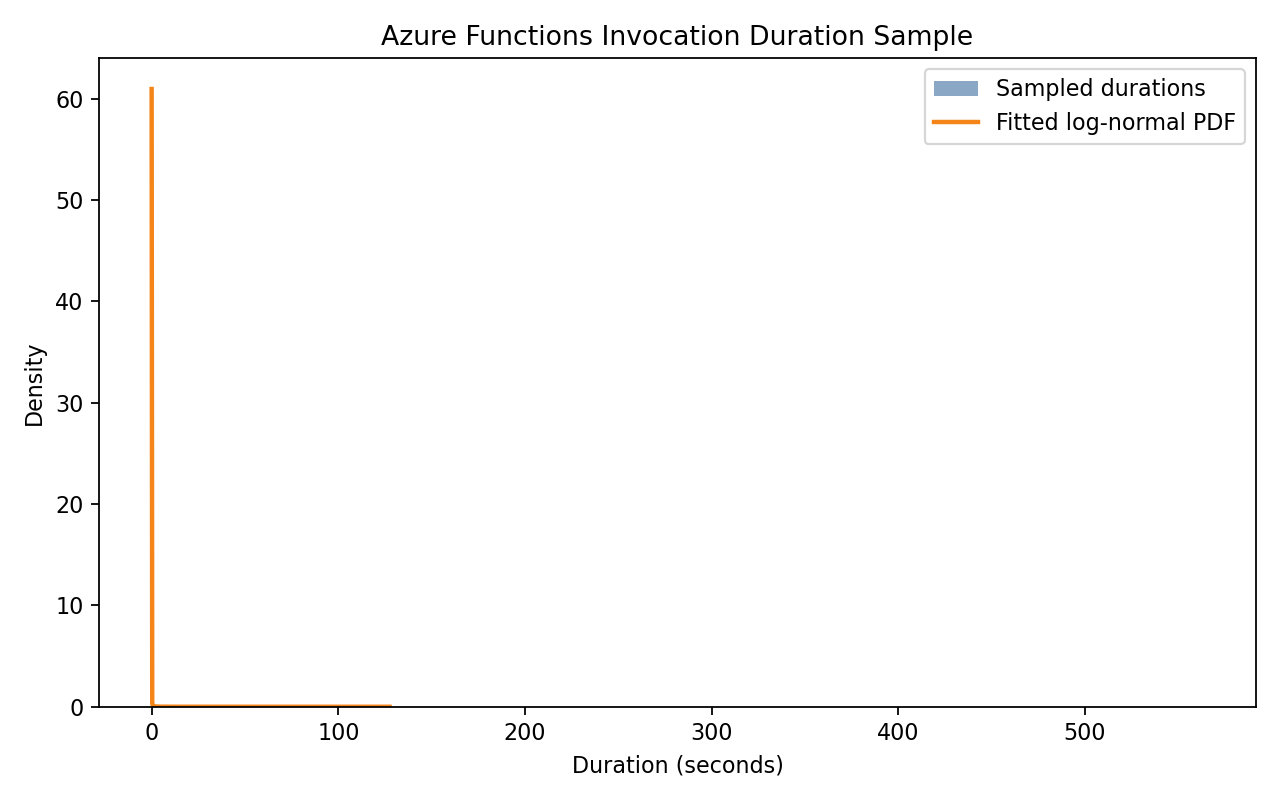
\includegraphics[width=0.72\textwidth]{azure_duration_histogram_fit.png}
\caption{Histogram of sampled Azure Functions invocation durations with a fitted log-normal density overlay. The raw duration distribution is extremely heavy-tailed, motivating the separate Azure-calibrated transfer test for cost-aware policies.}
\label{fig:azure_duration_hist}
\end{figure}

Two previously trained agents were evaluated without retraining: the base cost-aware \texttt{PPO-CostOnly} policy and the behavior-regularized warm-started PPO with $\lambda=0.1$. They were compared against the two strongest heuristics under the same Azure-derived PMF. Table~\ref{tab:azure_transfer} shows that the warm-started PPO transferred better than the plain cost-only PPO on all four standard scenarios. It achieved the best reward on \texttt{high\_load} and \texttt{oscillating}, while heuristics remained stronger on \texttt{low\_load} and \texttt{bursty}. This is a useful positive result: even though the learned policies were trained on a synthetic uniform distribution, behavior-regularized warm-starting improved robustness to a production-derived cost shift.

\begin{table}[H]
\centering
\caption{Zero-shot transfer under Azure-calibrated request costs. All policies were trained without Azure data and then evaluated under the empirical PMF derived from the Azure Functions trace. The regularized warm-start PPO transfers better than the plain cost-only PPO, especially on \texttt{high\_load} and \texttt{oscillating}.}
\label{tab:azure_transfer}
\resizebox{\textwidth}{!}{
\begin{tabular}{llcccccc}
\toprule
Scenario & Policy & Reward & Throughput & Latency & Drop Rate & HP Success & Budget Util. \\
\midrule
\multirow{4}{*}{low\_load}
& PPO-CostOnly & $16.886$ & $2.796$ & $7.397$ & $0.303$ & $0.496$ & $0.779$ \\
& PPO-WarmStart-Reg ($\lambda=0.1$) & $22.214$ & $2.828$ & $7.186$ & $0.299$ & $0.505$ & $0.784$ \\
& CostAwarePriority & $66.880$ & $2.769$ & $4.355$ & $0.304$ & $0.518$ & $0.775$ \\
& PriorityHeuristic & $49.490$ & $2.801$ & $5.586$ & $0.289$ & $0.503$ & $0.780$ \\
\midrule
\multirow{4}{*}{high\_load}
& PPO-CostOnly & $-208.662$ & $2.926$ & $7.787$ & $0.806$ & $0.839$ & $0.797$ \\
& PPO-WarmStart-Reg ($\lambda=0.1$) & $-90.955$ & $2.729$ & $4.612$ & $0.828$ & $0.811$ & $0.773$ \\
& CostAwarePriority & $-118.822$ & $2.910$ & $5.477$ & $0.807$ & $0.857$ & $0.795$ \\
& PriorityHeuristic & $-104.532$ & $2.872$ & $5.830$ & $0.815$ & $0.850$ & $0.788$ \\
\midrule
\multirow{4}{*}{bursty}
& PPO-CostOnly & $-124.311$ & $2.865$ & $6.890$ & $0.693$ & $0.731$ & $0.795$ \\
& PPO-WarmStart-Reg ($\lambda=0.1$) & $-62.056$ & $2.784$ & $5.463$ & $0.696$ & $0.721$ & $0.780$ \\
& CostAwarePriority & $-78.989$ & $2.985$ & $5.372$ & $0.670$ & $0.774$ & $0.802$ \\
& PriorityHeuristic & $-53.194$ & $2.903$ & $5.140$ & $0.681$ & $0.750$ & $0.792$ \\
\midrule
\multirow{4}{*}{oscillating}
& PPO-CostOnly & $-112.369$ & $2.878$ & $6.125$ & $0.730$ & $0.794$ & $0.790$ \\
& PPO-WarmStart-Reg ($\lambda=0.1$) & $-50.857$ & $2.736$ & $4.453$ & $0.748$ & $0.789$ & $0.774$ \\
& CostAwarePriority & $-68.661$ & $2.946$ & $5.024$ & $0.712$ & $0.808$ & $0.797$ \\
& PriorityHeuristic & $-61.186$ & $2.845$ & $5.004$ & $0.729$ & $0.814$ & $0.784$ \\
\bottomrule
\end{tabular}
}
\end{table}

\section{Discussion}
The experiments highlight one central lesson: reward alignment matters more than algorithm choice in this environment. The naive cost-aware reward collapsed because the agent was constrained by cost but rewarded mainly by request count. That created severe credit-assignment noise. Serving a few cheap requests could look superficially good under one part of the reward while still causing congestion penalties elsewhere, and the agent eventually converged to a degenerate low-admission strategy. Once the positive signal was changed to processed cost, the optimization target became congruent with the environment's real constraint. Stability improved immediately.

The warm-start experiments add a second lesson: imitation alone is not enough, but it is useful. Behavioral cloning transferred a large fraction of the heuristic's competence into the PPO policy. Standard PPO fine-tuning then destroyed that cloned behavior, demonstrating that warm-starting without policy regularization is unsafe in this domain. Behavior-regularized PPO fixed that specific failure mode. It did not make PPO dominant over heuristics, but it turned warm-starting into a stable and reproducible procedure.

The second lesson is that heuristics remain strong in structured domains. The cost-aware heuristics directly encode assumptions about priority, cost pressure, and queue growth. PPO, by contrast, must discover those relationships from sampled interaction. With limited training and a discrete action space, it is unsurprising that the learned controller remains competitive rather than dominant. This is a common RL pattern in constrained combinatorial settings: hand-crafted policies exploit inductive bias for free, whereas learned policies pay a sample-efficiency tax.

The OOD results sharpen this point. The cost-aware PPO generalized well to \texttt{cheap\_flood}, where many inexpensive requests are easy to pack into the budget. But it failed badly on \texttt{expensive\_attack}, where a few large-cost requests distort the training distribution. The policy trained on uniform costs from $1$ to $5$ did not learn a sufficiently abstract notion of cost packing. Instead, it overfit to the scale seen in training. This is a classic distribution-shift failure of pure model-free RL.

The Azure-calibrated transfer test refines that observation. When evaluated under a production-derived cost PMF, all policies degraded substantially because the distribution was far more skewed than the synthetic uniform costs used during training. However, the behavior-regularized warm-start PPO was more robust than the plain cost-only PPO across all four scenarios and even achieved the best reward on Azure-calibrated \texttt{high\_load} and \texttt{oscillating}. This suggests that heuristic imitation does not just stabilize PPO training; it also provides a better inductive bias under realistic cost shifts.

There is also a genuine systems trade-off in the final cost-aware policy. It serves fewer requests than the count-blind PPO, but it uses almost all of the budget and explicitly optimizes useful computational work rather than raw admissions. In a production setting where compute is the real bottleneck, this behavior may be preferable. That is, lower request throughput is not automatically worse if the served workload is more computationally valuable.

Finally, neither specialization nor warm-starting fully solved the gap to the strongest heuristics. High-load heuristic controllers still encoded domain structure more effectively than PPO learned from interaction. To surpass them, the agent would likely need richer feature engineering, more expressive actions, value-aware objectives, or online adaptation. Those are natural next steps, but they were beyond the scope of this project.

\section{Conclusion and Future Work}
This project extended a PPO-based API gateway rate limiter from a class-based count environment to a cost-aware admission-control setting. The main scientific contribution is not merely the environment extension itself, but the demonstration that reward design determines whether learning succeeds at all. A naive cost-aware reward caused policy collapse. Replacing the count-throughput term with a cost-served objective stabilized training and produced a high-utilisation cost-aware policy.

Three conclusions follow. First, reward design is critical in constrained RL systems. Second, RL can learn a stable and meaningful cost-aware admission controller that uses the processing budget aggressively and consistently. Third, strong heuristics remain difficult baselines to beat, particularly under adversarial or unseen cost distributions.

The warm-start extension refines the second conclusion: heuristic demonstrations can be transferred into PPO through behavioral cloning, and behavior-regularized PPO can preserve that initialization during fine-tuning. This is a useful algorithmic contribution even though the resulting policy still did not outperform the strongest teacher heuristic overall.

The Azure integration adds a final practical conclusion: evaluating only on synthetic cost distributions can overstate robustness. A production-derived cost PMF revealed a much harsher operating regime, but also showed that the regularized warm-start PPO transferred better than the plain cost-only agent.

Future work should explore policies that adapt online to new cost regimes, integrate more realistic resource accounting, coordinate across multiple gateways, and impose explicit safety constraints for service-level objectives. More broadly, the project suggests that the most promising route is not blindly scaling PPO, but combining learning with stronger structural priors about how expensive requests should be packed under limited budget.

\appendix
\section{Reproducibility and Artifacts}
The project was implemented as an extension of the existing reinforcement-learning course project repository. The main artifacts generated during experimentation include:
\begin{itemize}[leftmargin=1.5em]
    \item count-based ablation summaries,
    \item cost-aware screening outputs,
    \item full cost-aware comparisons,
    \item fine-tuning checkpoints and evaluation files,
    \item warm-start behavioral cloning and regularized PPO runs,
    \item Azure trace cost-profile extraction and transfer-evaluation outputs,
    \item narrative documents explaining experimental outcomes.
\end{itemize}

The important implementation principle was minimal refactoring: the PPO pipeline, plotting functions, and evaluation scripts were preserved wherever possible, and only the environment, reward, and heuristic logic were extended for cost-awareness.

\section{Additional Hyperparameters for Fine-Tuning}
\begin{table}[H]
\centering
\caption{Additional hyperparameters used in the high-load fine-tuning stage.}
\begin{tabular}{ll}
\toprule
Parameter & Value \\
\midrule
Base training episodes & $260$ \\
Fine-tuning episodes & $30$ \\
Fine-tuning actor learning rate & $0.0075$ \\
Fine-tuning critic learning rate & $0.0100$ \\
Validation scenario & \texttt{high\_load} \\
Validation frequency & every $10$ episodes \\
Checkpoint selection & best validation reward \\
\bottomrule
\end{tabular}
\end{table}

\section{Included Figure Files}
This report package includes the following copied plot assets under \texttt{figures/}:
\begin{itemize}[leftmargin=1.5em]
    \item \texttt{count\_training\_curves.png}
    \item \texttt{count\_high\_load\_throughput.png}
    \item \texttt{count\_high\_load\_hp\_success.png}
    \item \texttt{naive\_cost\_training\_curves.png}
    \item \texttt{cost\_high\_load\_throughput.png}
    \item \texttt{cost\_high\_load\_latency.png}
    \item \texttt{cost\_high\_load\_served\_cost.png}
    \item \texttt{cost\_high\_load\_budget\_utilization.png}
    \item \texttt{cost\_cheap\_flood\_throughput.png}
    \item \texttt{cost\_cheap\_flood\_budget\_utilization.png}
    \item \texttt{cost\_expensive\_attack\_latency.png}
    \item \texttt{azure\_duration\_histogram\_fit.png}
\end{itemize}

\end{document}
